% !TeX root = ../Book1.tex
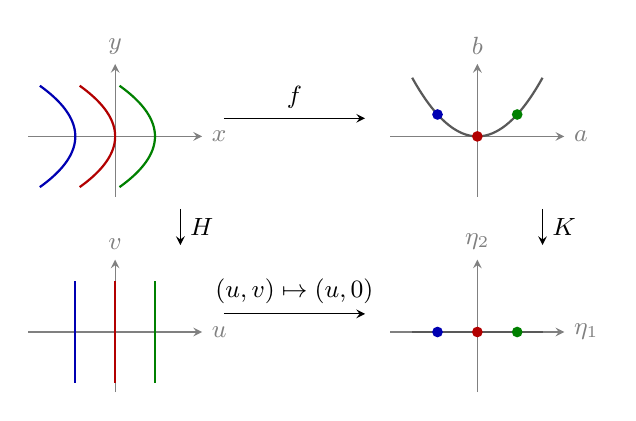
\begin{tikzpicture}[>=stealth,font=\small,scale=.92]
	\begin{scope}[yshift=2.7cm]
		\draw[->,gray] (-1.2,0)--(1.2,0) node[right] {\(x\)};
		\draw[->,gray] (0,-.83)--(0,1) node[above] {\(y\)};
		\foreach \level/\linecolour in {-.55/blue!70!black,0/red!70!black,.55/green!50!black}{
			\draw[thick,\linecolour,domain=-.7:.7,samples=40,variable=\t] plot ({\level-\t*\t},\t);
		}
	\end{scope}
	\begin{scope}[xshift=5cm,yshift=2.7cm]
		\draw[->,gray] (-1.2,0)--(1.2,0) node[right] {\(a\)};
		\draw[->,gray] (0,-.83)--(0,1) node[above] {\(b\)};
		\draw[thick,gray!70!black,domain=-.9:.9,samples=40] plot (\x,{\x*\x});
		\foreach \level/\linecolour in {-.55/blue!70!black,0/red!70!black,.55/green!50!black}{
			\fill[\linecolour] (\level,{\level*\level}) circle (2.1pt);
		}
	\end{scope}
	\draw[->] (1.5,2.95)--(3.45,2.95) node[midway,above] {\(f\)};
	\draw[->] (.9,1.7)--(.9,1.2) node[midway,right] {\(H\)};
	\draw[->] (5.9,1.7)--(5.9,1.2) node[midway,right] {\(K\)};
	\begin{scope}
		\draw[->,gray] (-1.2,0)--(1.2,0) node[right] {\(u\)};
		\draw[->,gray] (0,-.83)--(0,1) node[above] {\(v\)};
		\foreach \level/\linecolour in {-.55/blue!70!black,0/red!70!black,.55/green!50!black}{
			\draw[thick,\linecolour] (\level,-.7)--(\level,.7);
		}
	\end{scope}
	\begin{scope}[xshift=5cm]
		\draw[->,gray] (-1.2,0)--(1.2,0) node[right] {\(\eta_1\)};
		\draw[->,gray] (0,-.83)--(0,1) node[above] {\(\eta_2\)};
		\draw[thick,gray!70!black] (-.9,0)--(.9,0);
		\foreach \level/\linecolour in {-.55/blue!70!black,0/red!70!black,.55/green!50!black}{
			\fill[\linecolour] (\level,0) circle (2.1pt);
		}
	\end{scope}
	\draw[->] (1.5,.25)--(3.45,.25) node[midway,above] {\((u,v)\mapsto(u,0)\)};
\end{tikzpicture}

